\chapter{Lab Techniques I: Safety, Measurement and Separation}\label{ch:b1:lab-techniques-1}

Two students recrystallise the same batch of aspirin and measure its
melting point on the same heated bench. One reads \qty{134}{\celsius}, the
other \qty{136}{\celsius}. Do they disagree? Is the product pure? Neither
question can be answered from the two numbers alone: a measurement is
worth something only with its uncertainty, and a comparison only with a
rule. This last chapter gathers the practical side of the year: how to
read the \omterm{def:b1:lab-techniques-1:hazard}{hazards} of what is on the bench, how to state a measured value
and its uncertainty and compare it with another, and how the classic
operations of the organic laboratory --- extraction, filtration,
\omterm{def:b1:lab-techniques-1:recrystallisation}{recrystallisation}, distillation --- separate a product from what
surrounds it, then check that it is pure.

\begin{recall}
\omterm{def:b1:precipitation:solubility}{Solubility} and \omterm{def:b1:intermolecular-forces-solvents:miscibility}{miscibility} from intermolecular forces, polar and apolar
solvents (\cref{ch:b1:intermolecular-forces-solvents}); burettes, pipettes
and the \omterm{def:b1:titration-methods:titration}{end point} of a \omterm{def:b1:titration-methods:titration}{titration} (\cref{ch:b1:titration-methods}). The
school volume (grade 10) introduced liquid--liquid extraction,
\omterm{def:b1:lab-techniques-1:recrystallisation}{recrystallisation}, thin-layer chromatography and the \omterm{def:b1:extent-q-and-k:fractional-extent}{yield} of a synthesis;
here they are given their numbers.
\end{recall}

\begin{omfigure}
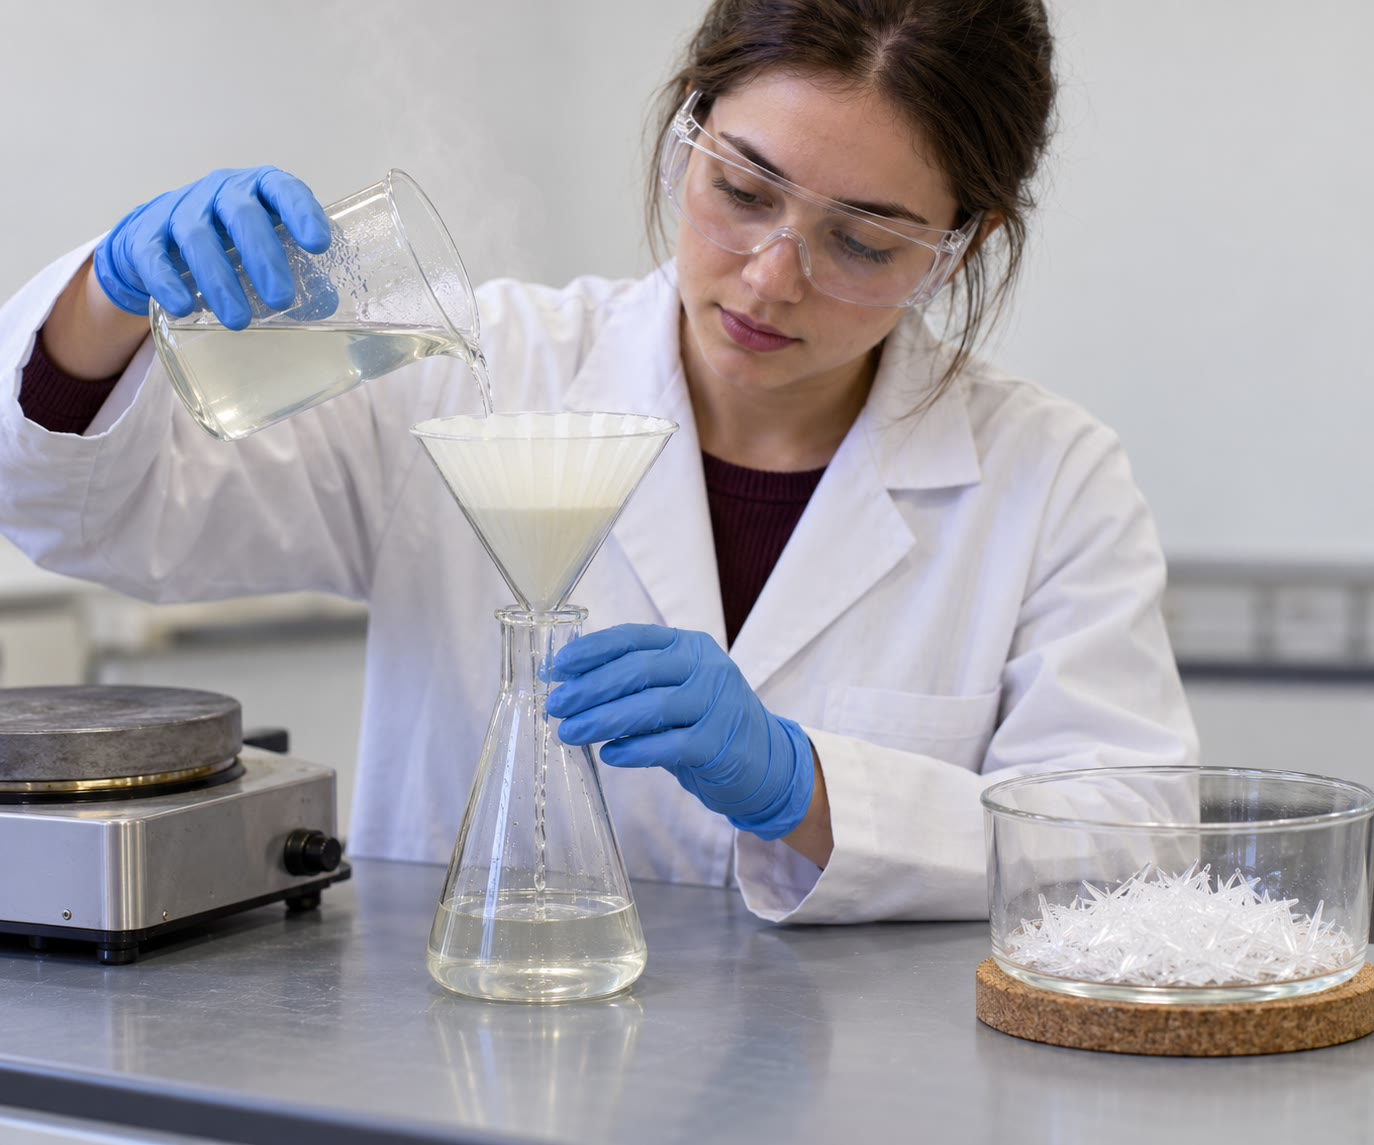
\includegraphics[width=0.5\linewidth]{images/book2/ai/b1-29-recrystallisation.jpg}

{\small Hot filtration during a \omterm{def:b1:lab-techniques-1:recrystallisation}{recrystallisation}: goggles, gloves and a
lab coat; the hot solution passes through a fluted filter paper, which
keeps back the insoluble impurities. Needles of a recrystallised product
wait in the dish on the right.}
\end{omfigure}

\section{Hazards and their labels}

\begin{definition}[Hazard and risk]\label{def:b1:lab-techniques-1:hazard}
A \emph{hazard}\index{hazard} is the intrinsic property of a substance (or
of a situation) that can cause harm: flammability, corrosiveness,
toxicity. The \emph{risk}\index{risk} is the likelihood that harm actually
occurs, and its severity, under the given conditions of use: it depends on
the hazard and on the exposure (quantity, concentration, duration, route,
protection).
\end{definition}

A \omterm{def:b1:lab-techniques-1:hazard}{hazard} cannot be changed without changing the substance; a \omterm{def:b1:lab-techniques-1:hazard}{risk} is
reduced by working on the exposure: a smaller quantity, a more dilute
solution, a fume cupboard, gloves and goggles, or a less hazardous reagent
for the same job.

\begin{definition}[GHS labelling]\label{def:b1:lab-techniques-1:ghs}
The labels of chemicals follow the Globally Harmonized System (GHS).
\begin{itemize}
  \item A \emph{hazard pictogram}\index{hazard pictogram} is a black symbol
        on a white diamond with a red border; there are nine, \texttt{GHS01}
        to \texttt{GHS09}.
  \item The \emph{signal word}\index{signal word} is \emph{Danger} for the
        more severe \omterm{def:b1:lab-techniques-1:hazard}{hazard} categories and \emph{Warning} for the less
        severe; a label carries one only, the more severe.
  \item A \emph{hazard statement}\index{hazard statement} is a standard
        phrase, coded H followed by three digits, describing a \omterm{def:b1:lab-techniques-1:hazard}{hazard}:
        H2xx physical \omterm{def:b1:lab-techniques-1:hazard}{hazards}, H3xx health \omterm{def:b1:lab-techniques-1:hazard}{hazards}, H4xx environmental
        \omterm{def:b1:lab-techniques-1:hazard}{hazards}.
  \item A \emph{precautionary statement}\index{precautionary statement},
        coded P and three digits, gives a measure to take: P1xx general,
        P2xx prevention, P3xx response, P4xx storage, P5xx disposal.
  \item The \emph{safety data sheet}\index{safety data sheet} is the
        document the supplier provides with a product, in standard
        sections: identification, \omterm{def:b1:lab-techniques-1:hazard}{hazards}, composition, first aid,
        fire fighting, handling and storage, exposure controls and
        protection, physical and chemical properties, stability, toxicity,
        disposal and transport.
\end{itemize}
\end{definition}

\begin{omfigure}
\setlength{\tabcolsep}{5pt}
\begin{tabular}{ccccc}
\begin{tabular}[t]{@{}c@{}}\ghs[1.25cm]{GHS01}\\[2pt]\footnotesize GHS01\\\footnotesize explosive\end{tabular} &
\begin{tabular}[t]{@{}c@{}}\ghs[1.25cm]{GHS02}\\[2pt]\footnotesize GHS02\\\footnotesize flammable\end{tabular} &
\begin{tabular}[t]{@{}c@{}}\ghs[1.25cm]{GHS03}\\[2pt]\footnotesize GHS03\\\footnotesize oxidising\end{tabular} &
\begin{tabular}[t]{@{}c@{}}\ghs[1.25cm]{GHS04}\\[2pt]\footnotesize GHS04\\\footnotesize gas under pressure\end{tabular} &
\begin{tabular}[t]{@{}c@{}}\ghs[1.25cm]{GHS05}\\[2pt]\footnotesize GHS05\\\footnotesize corrosive\end{tabular} \\[8pt]
\begin{tabular}[t]{@{}c@{}}\ghs[1.25cm]{GHS06}\\[2pt]\footnotesize GHS06\\\footnotesize acute toxicity\end{tabular} &
\begin{tabular}[t]{@{}c@{}}\ghs[1.25cm]{GHS07}\\[2pt]\footnotesize GHS07\\\footnotesize harmful, irritant\end{tabular} &
\begin{tabular}[t]{@{}c@{}}\ghs[1.25cm]{GHS08}\\[2pt]\footnotesize GHS08\\\footnotesize health hazard\end{tabular} &
\begin{tabular}[t]{@{}c@{}}\ghs[1.25cm]{GHS09}\\[2pt]\footnotesize GHS09\\\footnotesize environment\end{tabular} & \\
\end{tabular}

\smallskip
{\small The nine GHS pictograms: exploding bomb, flame, flame over circle,
gas cylinder, corrosion, skull and crossbones, exclamation mark, health
hazard (long-term effects: cancer, mutations, reproduction, sensitisation
of the airways, aspiration) and environment.}
% ledger: ghspic:GHS01, ghspic:GHS02, ghspic:GHS03, ghspic:GHS04,
% ghspic:GHS05, ghspic:GHS06, ghspic:GHS07, ghspic:GHS08, ghspic:GHS09
\end{omfigure}

\begin{example}[Reading the label of ethanol]
A bottle of ethanol carries the pictograms GHS02 and GHS07, the \omterm{def:b1:lab-techniques-1:ghs}{signal
word} \emph{Danger}, and the statements H225 (highly flammable liquid and
vapour, a physical \omterm{def:b1:lab-techniques-1:hazard}{hazard}, whose category calls for \emph{Danger}) and H319
(causes serious eye irritation, a health hazard, \emph{Warning} on its own).
Its \omterm{def:b1:lab-techniques-1:ghs}{precautionary statements} include P210 (keep away from heat, sparks and
open flames; no smoking), P233 (keep the container tightly closed), P280
(wear gloves and eye protection), P305+P351+P338 (if in eyes: rinse
cautiously with water for several minutes, remove contact lenses, continue
rinsing) and P403+P235 (store in a well-ventilated place, keep cool). The
practical consequences: no flame on the bench where ethanol is used,
goggles, a closed bottle.
\end{example}
% ledger: ghs:ethanol, hstat:H225, hstat:H319, pstat:P210, pstat:P233,
% pstat:P280, pstat:P305+P351+P338, pstat:P403+P235

\begin{method}[Preparing a session from the safety data sheets]\label{met:b1:lab-techniques-1:read-sds}
For each substance used or formed:
\begin{enumerate}
  \item read its pictograms, \omterm{def:b1:lab-techniques-1:ghs}{signal word} and H statements (section 2 of
        the sheet), and note the physical \omterm{def:b1:lab-techniques-1:hazard}{hazards} (fire, pressure,
        reactivity) apart from the health and environmental ones;
  \item for each operation (weighing, heating, transferring, filtering),
        estimate the exposure: quantity, state (a volatile liquid or a
        fine powder reaches the lungs), duration;
  \item choose the measures: substitution by a less hazardous reagent,
        smaller scale, fume cupboard, then personal protection (P2xx
        statements);
  \item plan the response to an incident (P3xx: eyes, skin, swallowing,
        fire) and where each waste goes (P5xx).
\end{enumerate}
\end{method}

\begin{inthelab}[Waste]
Nothing goes down the sink by default. Organic solvents are collected in
two containers, halogenated (dichloromethane, chloroform) and
non-halogenated (ethanol, propanone, cyclohexane, ethyl ethanoate), since
they are treated differently; aqueous acid and base solutions are
neutralised before disposal; solutions of heavy-metal ions (chromium,
copper, silver) have their own containers; broken glass and contaminated
solids are kept apart from ordinary rubbish. The statement P273, ``avoid
release to the environment'', on a label is a reminder that the waste
container, not the drain, is the end of the experiment.
% ledger: pstat:P273
\end{inthelab}

\section{Measurement and uncertainty}

A measured value is never the exact value of the quantity measured: repeat
the measurement and the result changes a little; read the scale and the
last digit is a guess. The uncertainty says how far from the measured
value the true value may reasonably lie.

\begin{definition}[Measurement uncertainty]\label{def:b1:lab-techniques-1:uncertainty}
\begin{itemize}
  \item The \emph{measurement uncertainty}\index{measurement uncertainty}
        is a parameter that characterises the dispersion of the values
        that can reasonably be attributed to the quantity measured.
  \item The \emph{standard uncertainty}\index{standard uncertainty} $u(x)$
        is that uncertainty expressed as a standard deviation.
  \item A \emph{type A evaluation}\index{type A evaluation} obtains $u$ by
        the statistical analysis of a series of repeated measurements; a
        \emph{type B evaluation}\index{type B evaluation} obtains it by any
        other means: the graduation of an instrument, the tolerance stated
        by its maker, a calibration certificate, the number of digits of a
        tabulated value.
  \item The \emph{expanded uncertainty}\index{expanded uncertainty}
        $U = k\,u$ is the standard uncertainty multiplied by a coverage
        factor $k$, usually $k = 2$; for a normal distribution the
        interval $x \pm 2u$ contains the true value with a probability of
        about \qty{95}{\percent}.
  \item The \emph{relative uncertainty}\index{relative uncertainty} is
        $u(x)/|x|$, often given in per cent.
\end{itemize}
\end{definition}

\begin{proposition}[Type A evaluation]\label{prop:b1:lab-techniques-1:type-a}
If $n$ independent measurements $x_1, \dots, x_n$ of the same quantity are
made, the best estimate is their mean $\bar x$; the experimental standard
deviation is
\[
  s = \sqrt{\frac{1}{n-1} \sum_{i=1}^{n} (x_i - \bar x)^2},
\]
and the \omterm{def:b1:lab-techniques-1:uncertainty}{standard uncertainty} of the mean is $u(\bar x) = s/\sqrt{n}$.
\end{proposition}
\begin{proof}[\omnameProof]
\emph{Admitted at this level}; the statistics of repeated measurements,
including the Student coefficient used when $n$ is small, are treated in
the Year 2 volume.
\end{proof}

\begin{omfigure}
\begin{tikzpicture}
\begin{axis}[width=7.4cm, height=5cm, xlabel={end-point volume (\unit{mL})},
  ylabel={number of readings}, ymin=0, ymax=8.5, xmin=12.2, xmax=12.7,
  xtick={12.2,12.3,12.4,12.5,12.6,12.7},
  xticklabel style={/pgf/number format/fixed, /pgf/number format/precision=1},
  axis lines=left, every axis plot/.append style={line join=round}]
  \addplot[ybar, bar width=0.045, fill=omDef!35, draw=omDef!80!black]
    table[x=V, y=count] {figdata/out/bachelor-1-type-a-uncertainty-a.dat};
  \addplot[omThm, thick, smooth]
    table[x=V, y=g] {figdata/out/bachelor-1-type-a-uncertainty-b.dat};
  \draw[omProp, thick, <->] (axis cs:12.384,7.6) -- (axis cs:12.526,7.6);
  \node[omProp, font=\small, above] at (axis cs:12.455,7.6) {$\bar V \pm s$};
\end{axis}
\end{tikzpicture}\hspace{0.6cm}%
\begin{tikzpicture}
\begin{axis}[width=5.6cm, height=5cm, xlabel={$x - x_0$}, ylabel={density},
  ymin=0, ymax=0.8, xmin=-1.6, xmax=1.6, xtick={-1,0,1},
  xticklabels={$-a$, $0$, $a$}, ytick={0.5}, yticklabels={$\frac{1}{2a}$},
  axis lines=left]
  \addplot[omDef!80!black, thick, fill=omDef!25] coordinates
    {(-1,0) (-1,0.5) (1,0.5) (1,0)} \closedcycle;
  \draw[omProp, thick, <->] (axis cs:-0.577,0.62) -- (axis cs:0.577,0.62);
  \node[omProp, font=\small, above] at (axis cs:0,0.62) {$\pm a/\sqrt3$};
\end{axis}
\end{tikzpicture}

{\small Left: twenty readings of the same \omterm{def:b1:titration-methods:titration}{titration} \omterm{def:b1:titration-methods:titration}{end point} (illustrative
data), read to \qty{0.05}{mL}, with the normal curve of the same mean
$\bar V = \qty{12.455}{mL}$ and standard deviation $s = \qty{0.071}{mL}$.
Right: the rectangular distribution of a \omterm{def:b1:lab-techniques-1:uncertainty}{type B evaluation}, a value known
only to lie between $x_0 - a$ and $x_0 + a$; its standard deviation is
$a/\sqrt3$.}
\end{omfigure}

\begin{example}[Twenty end points]
For the twenty readings of the figure, $\bar V = \qty{12.455}{mL}$,
$s = \qty{0.071}{mL}$ and $u(\bar V) = 0.071/\sqrt{20} = \qty{0.016}{mL}$.
One reading is uncertain by about $s$; the mean of twenty by about
$s/\sqrt{20}$, four and a half times less. The result is
$V = \qty{12.46}{mL}$ with $U = 2u = \qty{0.03}{mL}$.
\end{example}

\begin{proposition}[Type B evaluation for a rectangular distribution]\label{prop:b1:lab-techniques-1:type-b}
If all that is known of a quantity is that it lies, with equal
probability, anywhere between $x_0 - a$ and $x_0 + a$, its \omterm{def:b1:lab-techniques-1:uncertainty}{standard
uncertainty} is
\[
  u = \frac{a}{\sqrt3}.
\]
\end{proposition}
\begin{proof}
The probability density is $1/(2a)$ on $[x_0 - a, x_0 + a]$ and zero
elsewhere; its mean is $x_0$ by symmetry and its variance is
\[
  u^2 = \int_{x_0-a}^{x_0+a} (x - x_0)^2 \frac{\mathrm{d}x}{2a}
      = \frac{1}{2a} \left[\frac{t^3}{3}\right]_{-a}^{a}
      = \frac{1}{2a}\cdot\frac{2a^3}{3} = \frac{a^2}{3}. \qedhere
\]
\end{proof}

\begin{example}[A reading and a tolerance]
A burette graduated every \qty{0.1}{mL} is read to half a division: the
reading lies within $\pm\qty{0.05}{mL}$ of the value noted, so
$u = 0.05/\sqrt3 = \qty{0.029}{mL}$. A \qty{20}{mL} pipette whose maker
states a tolerance of $\pm\qty{0.03}{mL}$ delivers its volume with
$u = 0.03/\sqrt3 = \qty{0.017}{mL}$. A tabulated value given as
\qty{135}{\celsius} is known to $\pm\qty{0.5}{\celsius}$: $u = \qty{0.29}{\celsius}$.
\end{example}

\begin{proposition}[Combining uncertainties]\label{prop:b1:lab-techniques-1:combine}
For independent quantities: if $y = x_1 + x_2$ or $y = x_1 - x_2$, then
$u(y)^2 = u(x_1)^2 + u(x_2)^2$; if $y = x_1 x_2$ or $y = x_1/x_2$, then
\[
  \left(\frac{u(y)}{y}\right)^2 = \left(\frac{u(x_1)}{x_1}\right)^2
  + \left(\frac{u(x_2)}{x_2}\right)^2 .
\]
Several sources of uncertainty on the same quantity (a type A part and
type B parts) combine in the same way, as a sum of squares.
\end{proposition}
\admitted

The squares, not the uncertainties themselves, add: two independent
errors rarely push in the same direction at full size. A titrated volume
is a difference of two burette readings, so its reading uncertainty is
$\sqrt2 \times \qty{0.029}{mL} = \qty{0.041}{mL}$; and one large source of
uncertainty dominates the others, which is where an improvement should
be sought. The general rule, with partial derivatives, belongs to the
Year 2 volume.

\begin{method}[Reporting a result]\label{met:b1:lab-techniques-1:report-result}
\begin{enumerate}
  \item List the sources of uncertainty; evaluate each as a \omterm{def:b1:lab-techniques-1:uncertainty}{standard
        uncertainty} (type A from a series, type B as $a/\sqrt3$ from a
        half-width).
  \item Combine them as a sum of squares (\cref{prop:b1:lab-techniques-1:combine}).
  \item Give the \omterm{def:b1:lab-techniques-1:uncertainty}{expanded uncertainty} $U = 2u$ with one or two
        significant figures, and round the value to the same decimal
        place: $x = (\text{value} \pm U)$ unit, $k = 2$.
\end{enumerate}
\end{method}

\begin{definition}[Normalised deviation]\label{def:b1:lab-techniques-1:z-score}
The \emph{normalised deviation}\index{normalised deviation} (or $z$-score)
between two independent values $x_1$ and $x_2$ of the same quantity, of
standard uncertainties $u_1$ and $u_2$, is
\[
  z = \frac{|x_1 - x_2|}{\sqrt{u_1^2 + u_2^2}} .
\]
The two values are said to be compatible when $z \le 2$; a measured value
is compatible with a reference value under the same condition.
\end{definition}

\begin{example}[The two students]
The two melting points of the opening, \qty{134}{\celsius} and
\qty{136}{\celsius}, were each obtained with a \omterm{def:b1:lab-techniques-1:uncertainty}{standard uncertainty} of
\qty{0.8}{\celsius} (reading and calibration of the bench). Then
$z = 2/\sqrt{0.8^2 + 0.8^2} = 1.8 \le 2$: the students agree. Their mean,
\qty{135}{\celsius}, is also compatible with the tabulated melting point
of aspirin, \qty{135}{\celsius} under rapid heating. A tabulated value
given to the unit has $u = 0.5/\sqrt3 = \qty{0.29}{\celsius}$, so a single
reading with $u = \qty{0.8}{\celsius}$ is compatible with it while it lies
within $2\sqrt{0.8^2 + 0.29^2} = \qty{1.7}{\celsius}$ of it: a reading
below about \qty{133}{\celsius} would have pointed to an impure product.
\end{example}
% ledger: mp:aspirin

\section{Separating}

\begin{definition}[Partition coefficient]\label{def:b1:lab-techniques-1:partition-coefficient}
When a solute A is shared, at equilibrium, between two immiscible
solvents, an organic \omterm{def:b1:extent-q-and-k:system}{phase} and an aqueous \omterm{def:b1:extent-q-and-k:system}{phase}, the ratio of its
concentrations
\[
  K = \frac{[\mathrm{A}]_{\mathrm{org}}}{[\mathrm{A}]_{\mathrm{aq}}}
\]
is, for dilute solutions at a given temperature, a constant: the
\emph{partition coefficient}\index{partition coefficient} of A between the
two solvents.
\end{definition}

\begin{proposition}[Several extractions are better than one]\label{prop:b1:lab-techniques-1:multiple-extractions}
A volume $V_a$ of aqueous solution is extracted $n$ times, each time with a
fresh volume $V_o$ of organic solvent. The fraction of A left in the
aqueous \omterm{def:b1:extent-q-and-k:system}{phase} is
\[
  f_n = \left(1 + K \frac{V_o}{V_a}\right)^{-n}.
\]
For a fixed total volume of solvent, $n$ small portions extract more than
one large portion.
\end{proposition}
\begin{proof}
Let $m$ be the amount of A in the aqueous \omterm{def:b1:extent-q-and-k:system}{phase} before an extraction, and
$m'$ after. At equilibrium the organic \omterm{def:b1:extent-q-and-k:system}{phase} holds $m - m'$, and
$K = \dfrac{(m - m')/V_o}{m'/V_a}$, so $m - m' = K\dfrac{V_o}{V_a} m'$ and
$m' = m\big/\bigl(1 + K V_o/V_a\bigr)$. Each extraction multiplies the
amount left by the same factor; after $n$ of them, $f_n$ is the $n$-th
power. With a total volume $V$ split in $n$ portions $V/n$,
$\ln f_n = -n \ln(1 + KV/(nV_a))$; since $\ln(1+t)/t$ decreases with $t$,
$n \ln(1 + t/n)$ increases with $n$ for $t = KV/V_a > 0$, and $f_n$
decreases, towards the limit $\mathrm{e}^{-KV/V_a}$.
\end{proof}

\begin{example}[One portion or three]
A solute with $K = 4$ is extracted from \qty{100}{mL} of water with
\qty{60}{mL} of ethyl ethanoate. In one portion,
$f_1 = 1/(1 + 4 \times 0.6) = 0.29$: \qty{71}{\percent} is extracted. In
three portions of \qty{20}{mL}, $f_3 = (1 + 4 \times 0.2)^{-3} = 0.17$:
\qty{83}{\percent}. Ethyl ethanoate ($\rho = \qty{0.90}{g/cm^3}$) is the
upper layer in the separating funnel; dichloromethane
($\rho = \qty{1.33}{g/cm^3}$) would be the lower one.
\end{example}
% ledger: rho:ethyl-acetate, rho:CH2Cl2, rho:water

Filtration separates a solid from a liquid. By gravity, through a fluted
paper in a funnel, it keeps back an insoluble impurity from a hot solution
that must not cool on the way (hot filtration, as in the photograph at the
head of the chapter). Under reduced pressure, in a Büchner funnel on a
side-arm flask (as drawn in the school volume), it collects a solid
quickly and leaves it almost dry; the solid is washed on the filter with a
little cold solvent.

\begin{definition}[Recrystallisation]\label{def:b1:lab-techniques-1:recrystallisation}
\emph{Recrystallisation}\index{recrystallisation} purifies a solid by
dissolving it in the minimum of a hot solvent in which it is very soluble
hot and little soluble cold, then letting it crystallise on cooling; the
impurities either stay dissolved in the cold solvent (the mother liquor)
or, being insoluble, are removed beforehand by hot filtration.
\end{definition}

\begin{method}[Recrystallising a solid]\label{met:b1:lab-techniques-1:recrystallise}
\begin{enumerate}
  \item Choose the solvent: the product very soluble hot and little
        soluble cold, the soluble impurities soluble even cold, no
        reaction with the product, a boiling point below the product's
        melting point; a mixture of two \omterm{def:b1:intermolecular-forces-solvents:miscibility}{miscible} solvents (ethanol and
        water) can be tuned to the product.
  \item Dissolve the crude solid in the minimum of boiling solvent, added
        in small portions, under reflux if the solvent is volatile or
        flammable.
  \item If an insoluble impurity remains, filter hot.
  \item Let the solution cool slowly, then in ice: slow cooling gives
        larger, purer \omterm{def:b1:crystals-metals:crystal}{crystals}, which trap less mother liquor.
  \item Filter under reduced pressure, wash with a little ice-cold
        solvent, dry, weigh; check the purity (melting point, TLC).
\end{enumerate}
\end{method}

\begin{example}[The price of purity]
Aspirin dissolves in water at about \qty{3.3}{g/L} at \qty{25}{\celsius}
and \qty{10}{g/L} at \qty{37}{\celsius}, much more near the boiling
point. If \qty{40}{mL} of mother liquor and \qty{10}{mL} of washing water
leave the filter at \qty{25}{\celsius}, they carry away about
$\qty{0.050}{L} \times \qty{3.3}{g/L} = \qty{0.17}{g}$ of aspirin, whatever
its purity. Every millilitre of solvent beyond the minimum costs \omterm{def:b1:extent-q-and-k:fractional-extent}{yield}.
\end{example}
% ledger: sol:aspirin-25, sol:aspirin-37

A liquid is purified, or two liquids of well-separated boiling points are
separated, by \emph{simple distillation}: the mixture is boiled, the
vapour, richer in the more volatile component, is condensed and
collected. The temperature at the side arm is that of the vapour that
distils; while it stays constant, a pure substance is passing over.
Liquids of close boiling points need fractional distillation, a column
between the flask and the head, treated with the liquid--vapour diagrams
of the Year 2 volume.

\begin{omfigure}
\begin{tikzpicture}[font=\small, scale=0.95]
  \pic[transform shape] at (0,0) {heatingmantle};
  \pic[transform shape] at (0,0) {rbflask={0.45}{orange!25}};
  \foreach \x/\y in {-0.35/0.25,0.05/0.18,0.35/0.3}
    \fill[black!55] (\x,\y) circle (0.06);
  \pic[transform shape] (s) at (0,3.0) {stillhead};
  \pic[transform shape] at ($(s-top)+(0,-0.75)$) {thermometer};
  \pic[transform shape, rotate=-20] (c) at (s-arm) {liebig={3.4}};
  \coordinate (cend) at ($(s-arm)+(-20:3.4)$);
  \pic[transform shape] (a) at (cend) {adapter};
  \pic[transform shape] at ($(a-tip)+(0,-2.4)$) {erlenmeyer={0.22}{orange!12}};
  \draw[<-, omProp, thick] (0.12,3.72) -- (-1.4,4.4) node[left, text=black,
    align=right] {thermometer bulb\\ level with the side arm};
  \draw[<-, omProp, thick] ($(s-arm)+(-20:0.65)+(0.65,0.65)$) -- ++(0.2,0.9)
    node[above, text=black] {water out};
  \draw[<-, omProp, thick] ($(s-arm)+(-20:2.7)+(-0.2,-0.6)$) -- ++(0.05,-0.9)
    node[below, text=black] {water in};
  \draw[<-, omProp, thick] (-0.3,0.27) -- (-2.2,0.7) node[left, text=black]
    {boiling stones};
  \draw[<-, omProp, thick] (1.35,-0.6) -- (2.3,-1.1) node[right, text=black]
    {heating mantle};
  \draw[<-, omProp, thick] ($(a-tip)+(0.75,-2.0)$) -- ++(1.0,0.2)
    node[right, text=black] {distillate};
\end{tikzpicture}

{\small Simple distillation. The thermometer reads the temperature of the
vapour entering the condenser; cooling water enters at the low end of the
condenser so that the jacket stays full; the boiling stones prevent
violent bumping; the apparatus is open to the air at the receiver.}
\end{omfigure}

\begin{safety}{\ghs[5mm]{GHS02}}
A distillation apparatus is never closed: heated, a sealed system bursts.
Boiling stones are added to the cold liquid, never to a liquid already
hot (it may boil over at once). A flammable distillate is collected away
from any flame, the receiver if needed in ice.
\end{safety}

\section{Identifying and checking purity}

\begin{definition}[Retention factor]\label{def:b1:lab-techniques-1:retention-factor}
In thin-layer chromatography (TLC), a spot of the sample is deposited on
a baseline near the foot of a plate coated with a stationary \omterm{def:b1:extent-q-and-k:system}{phase}
(silica); the plate stands in a closed tank in a little eluent, which
rises through the coating by capillarity and carries the species at
different rates. The \emph{retention factor}\index{retention factor} of a
species is
\[
  R_f = \frac{\text{distance travelled by the spot}}
             {\text{distance travelled by the eluent front}},
\]
both measured from the baseline; $0 \le R_f \le 1$, and for given
stationary \omterm{def:b1:extent-q-and-k:system}{phase}, eluent and temperature it characterises the species.
\end{definition}

On polar silica, a polar species is held back more strongly than a less
polar one and has the smaller $R_f$; a more polar eluent moves every spot
further. Two species with the same $R_f$ on one plate may still differ;
two different $R_f$ prove them different. A pure product gives a single
spot.

\begin{omfigure}
\begin{tikzpicture}[font=\small, scale=1.7]
  \pic[transform shape] at (0,0) {tlcplate};
  \draw[omDef!80!black, densely dashed, line width=0.5pt] (-0.7,2.7) -- (0.7,2.7);
  \foreach \x in {-0.4,0,0.4} \fill[black!60] (\x,0.4) circle (0.025);
  \fill[omThm!70] (-0.4,{0.4+0.30*2.3}) ellipse (0.09 and 0.06);
  \fill[omDef!70] (0,{0.4+0.65*2.3}) ellipse (0.09 and 0.06);
  \fill[omThm!70] (0.4,{0.4+0.30*2.3}) ellipse (0.09 and 0.06);
  \fill[omDef!70] (0.4,{0.4+0.65*2.3}) ellipse (0.09 and 0.06);
  \node[below] at (-0.4,0) {A}; \node[below] at (0,0) {B};
  \node[below] at (0.4,0) {M};
  \draw[omProp, thick, |<->|] (0.95,0.4) -- (0.95,{0.4+0.65*2.3})
    node[midway, right] {$d_{\mathrm{B}}$};
  \draw[omProp, thick, |<->|] (1.55,0.4) -- (1.55,2.7)
    node[midway, right] {$d_{\mathrm{front}}$};
  \draw[omProp, thick, |<->|] (-0.95,0.4) -- (-0.95,{0.4+0.30*2.3})
    node[midway, left] {$d_{\mathrm{A}}$};
  \node[right, align=left, font=\footnotesize] at (0.75,2.85) {eluent front};
  \draw[omProp, thick, <-] (-0.6,0.4) -- (-1.2,0.05) node[left, text=black, font=\footnotesize] {baseline};
\end{tikzpicture}

{\small A developed TLC plate: references A and B and a mixture M,
deposited on the baseline. $R_f(\mathrm{A}) = d_{\mathrm{A}}/d_{\mathrm{front}}
= 0.30$, $R_f(\mathrm{B}) = 0.65$; the mixture shows both spots, at the
same heights.}
\end{omfigure}

\begin{method}[Running a TLC]\label{met:b1:lab-techniques-1:tlc}
\begin{enumerate}
  \item Draw the baseline in pencil about \qty{1}{cm} from the foot; deposit
        small spots of dilute solutions of the sample and of the references
        side by side.
  \item Put a few millimetres of eluent in the tank (below the baseline),
        close it, let the atmosphere saturate; stand the plate in it.
  \item Remove the plate when the front is about \qty{1}{cm} from the top;
        mark the front at once; dry.
  \item Reveal colourless spots (ultraviolet lamp on a fluorescent plate,
        iodine vapour, a stain); circle them in pencil.
  \item Measure the distances from the baseline and compute each $R_f$;
        compare the sample with the references on the same plate.
\end{enumerate}
\end{method}

\begin{omfigure}
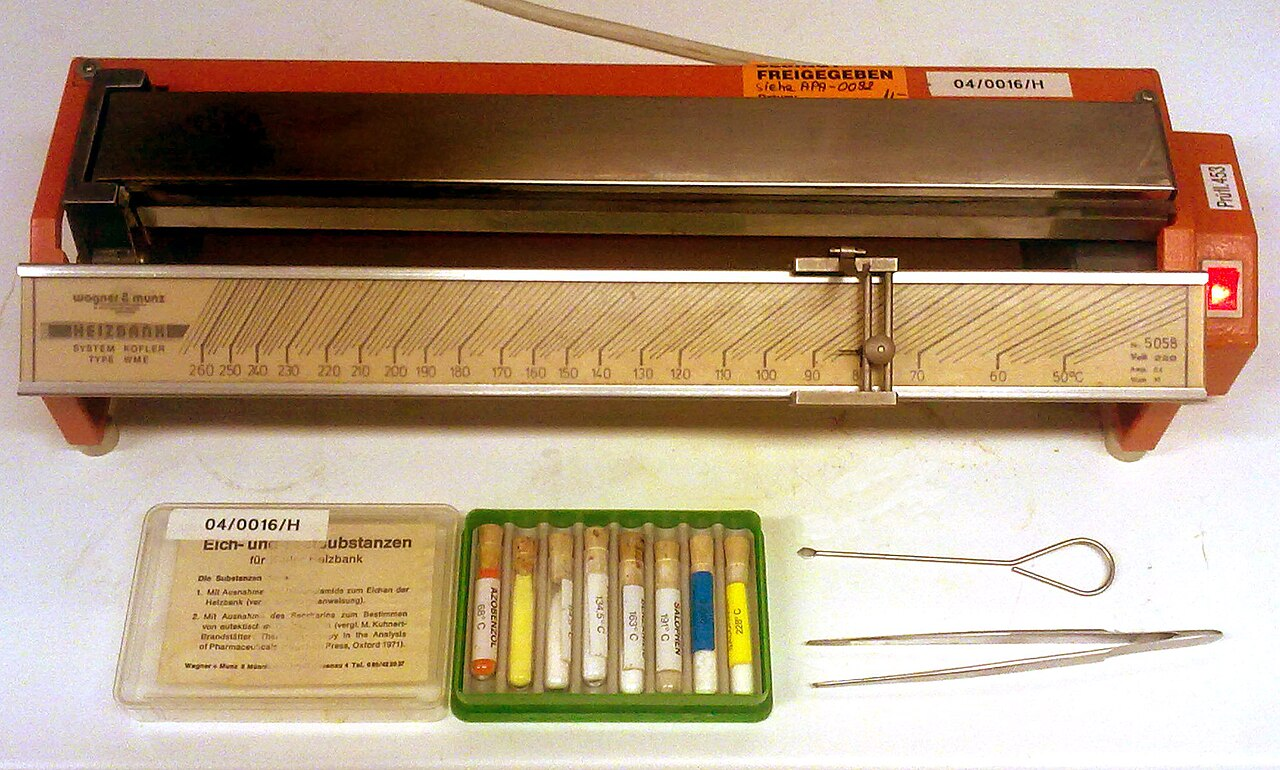
\includegraphics[width=0.62\linewidth]{images/book2/kofler-bench.jpg}

{\small A heated bench (Kofler bench): a metal strip heated at one end,
with a temperature gradient along it; the solid, sprinkled on the strip,
melts beyond a sharp line, read on the scale with the pointer. The box
holds reference substances of known melting point, used to calibrate it.
Photo: HBR, CC BY-SA 3.0, Wikimedia Commons.}
\end{omfigure}

\begin{method}[Measuring a melting point on a heated bench]\label{met:b1:lab-techniques-1:melting-point}
\begin{enumerate}
  \item Switch the bench on well in advance: the gradient takes time to
        settle.
  \item Calibrate it with a pure reference substance melting close to the
        expected value, sprinkled on the strip; set the pointer so that the
        scale reads its melting point on the line.
  \item Sprinkle a few \omterm{def:b1:crystals-metals:crystal}{crystals} of the dry sample from the cold end
        towards the hot end; push them back and forth with the spatula and
        set the pointer on the limit beyond which the solid melts at once.
  \item Read, repeat, clean the strip; take the mean of the readings and
        state the uncertainty (\cref{met:b1:lab-techniques-1:report-result}).
\end{enumerate}
\end{method}

A pure crystalline substance melts sharply at its melting point; an impure
one starts to melt lower and melts over a range of temperatures, because
the impurity lowers the temperature at which the solid and the liquid
coexist (the reason, the chemical potential of a solvent lowered by a
solute, is in the Year 2 volume). A melting point well below the
tabulated value, or a broad melting range, therefore reveals impurities;
a value compatible with the tabulated one, in the sense of the \omterm{def:b1:lab-techniques-1:z-score}{normalised
deviation}, supports purity without proving it.

\begin{inthelab}[Calibrating the bench]
The references are chosen to bracket the expected value. Acetanilide,
which melts at \qty{114.3}{\celsius}, and benzoic acid, at
\qty{122.4}{\celsius}, are classic standards for products melting between
\qty{110}{\celsius} and \qty{130}{\celsius}; for aspirin, a standard near
\qty{135}{\celsius} is better still. Aspirin itself decomposes as it melts,
so its observed melting point depends on how fast it is heated: tables give
\qty{135}{\celsius} for rapid heating, which is what a bench does.
% ledger: mp:acetanilide, mp:benzoic, mp:aspirin
\end{inthelab}

A liquid is identified, and its purity checked, by its \emph{refractive
index} $n_D$, the ratio of the speed of light in vacuum to its speed in the
liquid, measured with the yellow D line of sodium at a stated temperature
(usually \qty{20}{\celsius}), to four decimal places. Water has
$n_D = 1.333$, ethanol 1.3611 and cyclohexane 1.4266 at \qty{20}{\celsius}.
The index falls slightly as the temperature rises, so the instrument is
thermostatted.
% ledger: nD:water, nD:ethanol, nD:cyclohexane

\begin{omfigure}
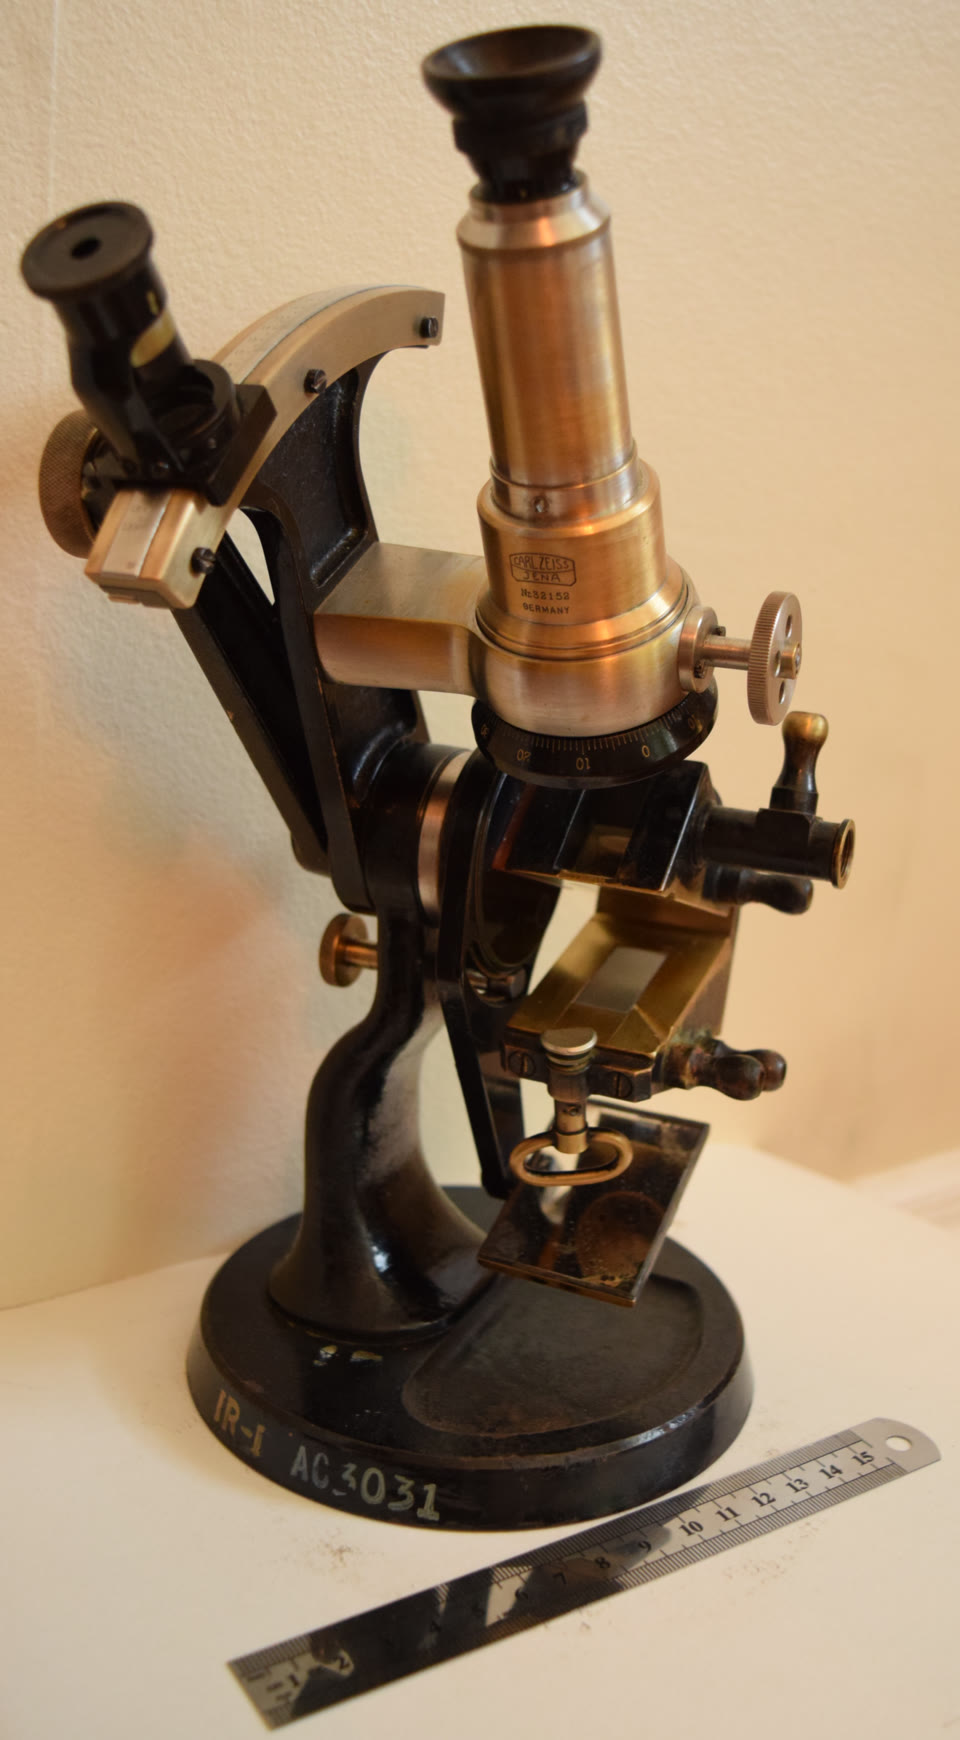
\includegraphics[height=6cm]{images/book2/abbe-refractometer.jpg}

{\small An Abbe refractometer: a drop of liquid is spread between two
prisms; the eyepiece shows a field half light and half dark, and the
boundary, set on the cross-hairs, gives the refractive index on the scale.
Photo: Foreade, CC BY-SA 4.0, Wikimedia Commons.}
\end{omfigure}

\section{Exercises}

\begin{exercise}[$\star$]\label{exo:b1:lab-techniques-1:1}
A bottle of propanone carries the pictograms GHS02 and GHS07 and the
statements H225, H319 and H336. Which \omterm{def:b1:lab-techniques-1:ghs}{signal word} does it carry? Which
statements describe a physical \omterm{def:b1:lab-techniques-1:hazard}{hazard}, which a health hazard? Name two
precautions they call for.
\end{exercise}

\begin{exercise}[$\star$]\label{exo:b1:lab-techniques-1:2}
\omterm{def:b1:lab-techniques-1:hazard}{Hazard} or \omterm{def:b1:lab-techniques-1:hazard}{risk}? (a) Concentrated sulfuric acid causes severe burns.
(b) Weighing \qty{50}{mg} of a toxic powder in a fume cupboard with
gloves exposes the operator little. (c) Sodium releases hydrogen with
water. (d) The same solvent is more dangerous used hot in an open beaker
than cold in a closed bottle.
\end{exercise}

\begin{exercise}[$\star$]\label{exo:b1:lab-techniques-1:3}
On a TLC plate the eluent front is \qty{6.0}{cm} above the baseline;
the sample gives spots at \qty{2.1}{cm} and \qty{4.2}{cm}. Compute their
$R_f$. A reference deposited on the same plate rises to \qty{4.2}{cm}:
what can and cannot be concluded?
\end{exercise}

\begin{exercise}[$\star$]\label{exo:b1:lab-techniques-1:4}
A burette graduated every \qty{0.1}{mL} is read to half a division.
Compute the \omterm{def:b1:lab-techniques-1:uncertainty}{standard uncertainty} of one reading, then of a delivered
volume, the difference of two readings.
\end{exercise}

\begin{exercise}[$\star\star$]\label{exo:b1:lab-techniques-1:5}
Five weighings of the same sample give \qty{0.2512}{g}, \qty{0.2508}{g},
\qty{0.2515}{g}, \qty{0.2510}{g} and \qty{0.2505}{g}. Compute the mean,
the experimental standard deviation, the \omterm{def:b1:lab-techniques-1:uncertainty}{standard uncertainty} of the mean,
and report the result with $k = 2$.
\end{exercise}

\begin{exercise}[$\star\star$]\label{exo:b1:lab-techniques-1:6}
A solute with \omterm{def:b1:lab-techniques-1:partition-coefficient}{partition coefficient} $K = 3$ between an organic solvent and
water is extracted from \qty{50}{mL} of water with \qty{30}{mL} of solvent
in total. Compute the fraction extracted in one portion, in two portions
of \qty{15}{mL}, and in three of \qty{10}{mL}.
\end{exercise}

\begin{exercise}[$\star\star$]\label{exo:b1:lab-techniques-1:7}
A \omterm{def:b1:titration-methods:titration}{titration} gives a concentration of \qty{0.1012}{mol/L} with \omterm{def:b1:lab-techniques-1:uncertainty}{standard
uncertainty} \qty{0.0006}{mol/L}; the solution was prepared at
\qty{0.1000}{mol/L} with \omterm{def:b1:lab-techniques-1:uncertainty}{standard uncertainty} \qty{0.0002}{mol/L}. Are the
two values compatible? What if the \omterm{def:b1:titration-methods:titration}{titration} uncertainty had been
\qty{0.0004}{mol/L}?
\end{exercise}

\begin{exercise}[$\star\star$]\label{exo:b1:lab-techniques-1:8}
The solubilities (illustrative values, \unit{g} per \qty{100}{mL}) of a
solid in three solvents are: solvent P, 1.5 cold and 2.0 boiling; solvent
Q, 0.3 cold and 12 boiling; solvent R, 9 cold and 25 boiling. Which
solvent suits a \omterm{def:b1:lab-techniques-1:recrystallisation}{recrystallisation}, and why not the other two? With the
right solvent, what is the largest fraction of \qty{5.0}{g} of the solid
that can be recovered, if the minimum of boiling solvent is used and the
mixture cooled?
\end{exercise}

\begin{exercise}[$\star\star$]\label{exo:b1:lab-techniques-1:9}
A colourless liquid, thermostatted at \qty{20}{\celsius}, has
$n_D = 1.3612$. Which of water, ethanol and cyclohexane can it be? Why is
the temperature stated? What would a value of 1.350 suggest?
\end{exercise}

\begin{exercise}[$\star\star\star$]\label{exo:b1:lab-techniques-1:10}
With the data of \cref{exo:b1:lab-techniques-1:6}, show that however
finely the \qty{30}{mL} of solvent is divided, at most a fraction
$1 - \mathrm{e}^{-KV/V_a}$ of the solute can be extracted, and compute it.
How many portions reach \qty{99}{\percent} of that limit?
\end{exercise}

\begin{exercise}[$\star\star\star$]\label{exo:b1:lab-techniques-1:11}
A quantity is known to lie between $x_0 - a$ and $x_0 + a$, values near
$x_0$ being more likely: its density is triangular, $(a - |x - x_0|)/a^2$.
Check that it is normalised and show that its \omterm{def:b1:lab-techniques-1:uncertainty}{standard uncertainty} is
$a/\sqrt6$. Compare with the rectangular case.
\end{exercise}

\begin{exercise}[$\star\star\star$]\label{exo:b1:lab-techniques-1:12}
A standard solution is made by dissolving the sample of
\cref{exo:b1:lab-techniques-1:5} (molar mass \qty{204.2}{g/mol}, its
uncertainty negligible) in a \qty{100.00}{mL} volumetric flask whose
volume has a \omterm{def:b1:lab-techniques-1:uncertainty}{standard uncertainty} of \qty{0.06}{mL}. Compute the
concentration and its relative and expanded uncertainties. Which source
dominates?
\end{exercise}

\section{Problem: Purifying Aspirin}

\begin{problem}[{Weekend problem --- the hazards of a synthesis, the
recrystallisation of crude aspirin and its yield, a melting point with its
type A and type B uncertainties, and the normalised deviation from the
tabulated value}]
\label{pb:b1:lab-techniques-1:1}
A student makes aspirin by heating \qty{2.00}{g} of salicylic acid with an
excess of ethanoic anhydride, then recrystallises the crude product.
Molar masses (\unit{g/mol}): salicylic acid \ce{C7H6O3} 138.0, aspirin
\ce{C9H8O4} 180.0, ethanoic anhydride \ce{C4H6O3} 102.0. Labels:
salicylic acid GHS05, GHS07, H302, H318; ethanoic anhydride GHS02,
GHS05, GHS06, GHS07, H226, H302, H314, H332; aspirin GHS07, H302.
\omterm{def:b1:precipitation:solubility}{Solubility} of aspirin in water: \qty{3.3}{g/L} at \qty{25}{\celsius}.
Tabulated melting point of aspirin (rapid heating): \qty{135}{\celsius}.
% ledger: ghs:salicylic, ghs:acetic-anhydride, ghs:aspirin, sol:aspirin-25,
% mp:aspirin, hstat:H318, hstat:H226, hstat:H314, hstat:H302

\medskip
\noindent\textbf{Part I --- \omterm{def:b1:lab-techniques-1:hazard}{Hazards}.}
\begin{enumerate}
  \item What does each pictogram on the label of ethanoic anhydride mean?
  \item Which \omterm{def:b1:lab-techniques-1:ghs}{signal word} does the label of salicylic acid carry? And that
        of aspirin?
  \item Ethanoic anhydride has the more severe \omterm{def:b1:lab-techniques-1:hazard}{hazards}. Explain how the
        \omterm{def:b1:lab-techniques-1:hazard}{risk} of handling \qty{5}{mL} of it can nevertheless be made small.
  \item Which of the anhydride's statements call for goggles and gloves,
        and which for the fume cupboard and the absence of flames?
  \item What is done at once if a drop of anhydride reaches an eye?
  \item The filtrate of the \omterm{def:b1:lab-techniques-1:recrystallisation}{recrystallisation} contains ethanoic acid and a
        little ethanol in water. Where does it go?
\end{enumerate}

\noindent\textbf{Part II --- Synthesis and \omterm{def:b1:lab-techniques-1:recrystallisation}{recrystallisation}.}
\begin{enumerate}[resume]
  \item Write the equation of the synthesis, with ethanoic acid
        \ce{C2H4O2} as by-product, and check that it is balanced.
  \item Compute the amount of salicylic acid and the maximum mass of
        aspirin.
  \item The crude dry product weighs \qty{2.41}{g}. Why can the
        \omterm{def:b1:lab-techniques-1:recrystallisation}{recrystallisation} not be skipped although this is
        \qty{92}{\percent} of the maximum?
  \item Aspirin is recrystallised from a little ethanol completed with hot
        water. Why is the \omterm{def:b1:precipitation:solubility}{solubility} in water at \qty{25}{\celsius}, compared
        with that near the boiling point, the property that matters?
  \item Why is the crude solid dissolved in the minimum of hot solvent?
  \item Why is the solution cooled slowly, then in ice?
  \item \qty{40}{mL} of filtrate at \qty{25}{\celsius} leave the funnel,
        then \qty{5}{mL} of washing water. Estimate the mass of aspirin
        lost with them.
  \item The pure dry product weighs \qty{1.95}{g}. Compute the \omterm{def:b1:extent-q-and-k:fractional-extent}{yield}.
\end{enumerate}

\noindent\textbf{Part III --- Melting point.}
\begin{enumerate}[resume]
  \item Six readings on the bench, calibrated just before, give 134, 135,
        133, 135, 134 and \qty{136}{\celsius}. Compute the mean.
  \item Compute the experimental standard deviation.
  \item Deduce the type A \omterm{def:b1:lab-techniques-1:uncertainty}{standard uncertainty} of the mean.
  \item Each reading is made to the nearest degree. Compute the type B
        uncertainty of reading.
  \item The calibration of the bench is guaranteed to within
        $\pm\qty{1}{\celsius}$. Compute the corresponding type B
        uncertainty, then the combined \omterm{def:b1:lab-techniques-1:uncertainty}{standard uncertainty}.
  \item Report the melting point with its \omterm{def:b1:lab-techniques-1:uncertainty}{expanded uncertainty} ($k = 2$).
  \item A classmate's crude product melts between 120 and
        \qty{128}{\celsius}. What does this indicate?
\end{enumerate}

\noindent\textbf{Part IV --- Comparison with the reference.}
\begin{enumerate}[resume]
  \item The tabulated value is given to the unit. What \omterm{def:b1:lab-techniques-1:uncertainty}{standard
        uncertainty} does that imply?
  \item On a TLC plate (front \qty{6.0}{cm}), the crude product shows
        spots at \qty{2.3}{cm} and \qty{3.3}{cm}, salicylic acid one spot
        at \qty{2.3}{cm}, the recrystallised product one spot at
        \qty{3.3}{cm}. Compute the $R_f$ values and conclude.
  \item Why does the melting point of aspirin depend on the heating rate?
  \item Compute the \omterm{def:b1:lab-techniques-1:z-score}{normalised deviation} $z$ between the measured and the
        tabulated melting points, and say whether they are compatible.
\end{enumerate}
\end{problem}
